\documentclass{gmto}

\usepackage{color,amsmath,amssymb,xspace}
\usepackage{booktabs}

\DocID{GMT-XXX-\#\#\#\#}
\DocVersion{1.0}
\DocStatus{Draft}

\addbibresource{gmt.bib}
\graphicspath{{figures/}}

\title{Environmental conditions for simulations}
%\subtitle{}
\author{R. Conan}
\date{\today}

\newtheorem{theorem}{Definition}
\def\PSSn{\ensuremath{\mathrm{PSSn}\left( \vec\theta,T \right)}}
\def\median{\ensuremath{\mathrm{median}}}

\begin{document}

\maketitle

\clearpage

\section*{Signatures}
\vspace{1cm}
\subsection*{Author}
\vspace{1.5cm}
%\tabulinesep=1em
\begin{tabu} to \linewidth {X[3,l]X[1,l]}
  \rule{\linewidth}{.1pt} & \rule{\linewidth}{.1pt} \\
  Name, title & Date
\end{tabu}
\vspace{1.5cm}
\subsection*{Approvers}
\vspace{1.5cm}
%\tabulinesep=1em
\begin{tabu} to \linewidth {X[3,l]X[1,l]}
  \rule{\linewidth}{.1pt} & \rule{\linewidth}{.1pt} \\
  Name, title & Date \\[1cm]
  \rule{\linewidth}{.1pt} & \rule{\linewidth}{.1pt} \\
  Name, title & Date
\end{tabu}

\clearpage

\section*{Revision Log}

\begin{revisions}
  1.0 & \today & All & None & Initial version & Author \\  
\end{revisions}

\clearpage

\tableofcontents
\listoffigures
\listoftables

\clearpage

\section{Purpose}
\label{sec:purpose}

The purpose of the document is to define and to catalog all the environmental
parameters that an integrated simulation may need.
The goal being that all the simulations pull the environmental parameters from a
single source that is this document and its data archive companion.

\section{Introduction}
\label{sec:introduction}

To ensure that the scientific goals of the Observatory are met, Key Performance
Parameters $($KPPs$)$ are used to measure the technical performance of the GMT.
These KPPs have been used to prioritize maturation plans for technologies and
novel system-level designs.
A set of KPPs have been defined to assess the performance of the telescope
through Assembly, Integration, Verification, and Commissioning $($AIVC$)$, while
other sets are used to measure instrument performances as their commissioning is
being completed.
Each KPP has a threshold value that represents a minimum acceptable performance and an objective value that represents the desired operational performance. 

The KPPs for GMT are: throughput; on-axis image quality; image quality spatial
variability though the field of view; image quality temporal stability;
effective collecting area; and target acquisition time. The first five listed
are related to observatory performance while the last is a probe of observatory
efficiency. The metric that assess image quality at a given location if the
field $\vec\theta$ and for a given exposure time $T$ is the normalized point
source sensitivity: \PSSn.

Each KPP is derived from key science capabilities that are defined at the SRD
level. Key science drivers include on-axis sensitivity, image quality, image
quality variation, relative photometric accuracy, and astrometric accuracy.
Each of the science driver was decomposed into its major contributors.
For instance, on-axis sensitivity is affected by sky brightness, telescope
thermal background, throughput, pupil stability, image quality, image quality
temporal stability, and the effective collecting area of the telescope.
Both astrometric variation and relative photometric accuracy are both also
affected by image quality and image quality temporal variation. 

The Key Performance Parameters are defined as follows: 
\begin{description}
\item[On-Axis PSSn] The median Normalized Point Source Sensitivity at the telescope focal plane and over 900 s integrations. The
  on-axis PSSN is a median over time. The PSSN in Natural Seeing performance
  modes is derived from the ConOps Image Quality Efficiency Metric requirements.
  The PSSN in GL performance modes is derived from the SRD Image Quality
  specification of the parent OC. Each value is referenced to the median image
  quality of the free atmosphere calculated from DIMM seeing ($\theta$ = 0.63
  arcsec) with an assumed outer scale ($L_0$ = 25 m). The Image Quality Flow
  Down Analysis document $[$GMT-DOC-03033$]$ describes the derivation of the
  PSSN requirements for both modes.
  \begin{theorem}
    $\mathrm{KPP} = \median\left( \mathrm{PSSn}(0,900) \right)$
  \end{theorem}
  
\item[PSSn Spatial Uniformity] The peak-to-valley uniformity of the PSSN across the field of view at the telescope focal plane expressed as a percent difference from the mean PSSN. This is a direct flow-down from the Image Quality Variation of the parent OC. PSSN uniformity variation from inherent design astigmatism is not included as it is a static effect that is calibratable.  
  \begin{theorem}
    \begin{displaymath}
    \mathrm{KPP} = \median\left( 100
      {\max_{\vec\theta}\left[\mathrm{PSSn}(\vec\theta,900)\right]-\min_{\vec\theta}\left[\mathrm{PSSn}(\vec\theta,900)\right]\over\left\langle
       \mathrm{PSSn}(\vec\theta,900) \right\rangle_{\vec\theta}} \right)
    \end{displaymath}
  \end{theorem}

\item[Wavefront Error]: The on-axis RMS wavefront error at the telescope exit pupil plane expressed in nanometers, median over time and over 120 s integrations. The flow-down from the Image Quality and Strehl Ratio for OPMs 7 and 8 is described in the Adaptive Optics Image Quality Budgets (GMT-AO-REF-00518). The flow-down from Contrast in OPM 9 has not yet been completed.  

\item[Throughput]: The on-axis, minimum allotted throughput of the telescope averaged over a 50 nm bandpass at central wavelengths of astronomical filters (U, B, V, R, I, z, J, H, K). It does not include the throughput of the atmosphere or instruments. Values assume the primary and secondary mirrors are coated with bare aluminum and that the tertiary mirror (for diffraction-limited modes) is coated in 4-layer protected Gemini silver (see Boccas et al. 2004). The flow-down from the On-Axis Sensitivity specification of the parent OC is described in GMT-DOC-03229.  

\item[PSSN Temporal Stability]: The median over field position of the
  peak-to-valley temporal change in the PSSN over a 2-hour period (8 $\times$
  900 exposures), excluding throughput variations (i.e., due to
  atmosphere-induced changes in the PSSN) expressed as a percent difference from
  the mean PSSN over time. The 2-hour period represents an estimate of the time
  between taking PSF standard stars during spectroscopic observations. This is a
  direct flow-down from the Relative Photometric Error of the parent OC,
  assuming aperture photometry is used  %\marginpar{What about atmosphere variability?}
  \begin{theorem}
    \begin{displaymath}
    \mathrm{KPP} = \median\left( 100
      {\max_{\vec\theta}\left[\widehat{\mathrm{PSSn}}(\vec\theta,900)\right]-\min_{\vec\theta}\left[\widehat{\mathrm{PSSn}}(\vec\theta,900)\right]\over\left\langle
       \widehat{\mathrm{PSSn}}(\vec\theta,900) \right\rangle_{\vec\theta}} \right)   
\end{displaymath}
with
\begin{displaymath}
  \widehat{\mathrm{PSSn}}(\vec\theta,900) = \median_{2h}\left( \mathrm{PSSn}(\vec\theta,900) \right)
\end{displaymath}

  \end{theorem}

\item[Target Acquisition]: The maximum time to acquire a new target using any deployed instrument. This is a direct flow-down from the ConOps. The time is calculated from the start of a slew to the start of centering on the science instrument and includes closing any wavefront control and alignment loops.

\item[Effective Collecting Area]: Minimum total collecting area of the observatory configuration given in square meters. The value is related to the total number of available segments. Note that the center segment will contribute the least amount of effective collecting area given the center hole and the obscuration from the secondary and its support trusses. The total number of segments is directly related to the overall sensitivity. 
\end{description}

\section{Image quality metrics}
\label{sec:perf-metrics}

The image quality that the telescope must deliver is first defined in the
Science Requirement Document (SRD\cite{SRD}) and it is expressed in
terms of the Full Width at Half Maximum (FWHM) of an image for different observing cases.
The Observatory Requirements Document (ORD\cite{ORD}) divides the observing conditions
into observing performance modes (OPM) and assign to each OPM a new metric, the
PSSn\cite{SNA+2009}.

Both metrics describe the effects of different type of aberrationss on an image.
The PSSn is very little sensitive to low frequency spatial aberrations, but low frequency aberrations have a more significant impact on the FWHM
as they contribute mostly to the blur of the image core.
On the other hand, high frequency aberrations create distortions in the tail of
the PSF and have very little influence on the FWHM but will show more
significantly in the PSSn.
Consequently both metrics are needed in order to fully specify image quality of
a given OPM.

In the following,we will refer to $I(\vec\alpha,\vec \theta, t)$ as the
intensity distribution in the focal plane of the telescope of an unresolved
object or point spread function (PSF) at time $t$.
$\vec\alpha$ denotes the angular coordinate in the focal plane with origin
$\vec\theta$.
$\vec \theta$ is also the pointing vector of the telescope.

The optical transfer function $O$ of the telescope (OTF) is obtained as the Fourier transfer of
$I$:
\begin{equation}
  O(\vec\rho)=\mathcal{F}\left[ I(\vec\alpha) \right](\vec \rho) = \iint I(\vec\alpha) \exp\left( 2i\pi \vec\alpha\cdot\vec\rho \right)\mathrm{d}^2\vec\alpha.
  \label{eq:16}
\end{equation}

\subsection{Full Width at Half Maximum}
\label{sec:fwhm-def}

\def\psf{\mathrm{psf}}
\def\otf{\mathrm{otf}}
The FWHM ($\varepsilon$) is defined as:
\begin{equation}
  \label{eq:13}
  I(\varepsilon/2,\gamma) =  I(0)/2.
\end{equation}
As shown in Eq.~\eqref{eq:13}, the FWHM is a function of the polar angle $\gamma$
in the focal plane as an image is not always centro--symmetric.
So instead, we will define ($\varepsilon$) with the following expression:
\begin{equation}
  \label{eq:14}
  {1\over 2\pi}\int_0^{2\pi}I(\varepsilon/2,\gamma)\ \mathrm{d}\gamma =  I(0)/2,  
\end{equation}
where now the FWHM is defined for the circular average of the image.
The numerical computation of $\varepsilon$ from a discrete image can be quite
cumbersome and we will compute it instead from the OTF.
Inserting Eq.~\eqref{eq:16} into Eq.~\eqref{eq:14} and integrating over $\gamma$
lead to $\varepsilon$ beeing the root of the following scalar equation:
\begin{equation}
  \label{eq:15}
  \iint \Re\left(O(x,y)\right) \left(1 - 2J_0(\pi\varepsilon\rho)\right)\mathrm{d}x\mathrm{d}y = 0, \quad\vec\rho(x,y).
\end{equation}


\subsection{PSSn definition}
\label{sec:pssn-def}

The $\mathrm{PSSn}$ is written as
\begin{equation}
  \label{eq:1}
\mathrm{PSSn} = {\displaystyle\iint {\mathrm d}^2\vec\alpha \left| \int_0^T I(\vec\alpha,\vec \theta, t){\mathrm d}t \right|^2 \over \displaystyle\iint {\mathrm d}^2\vec\alpha \left| I_0(\vec\alpha,\vec \theta) \right|^2},
\end{equation}
where $T$ is the
integration or exposure time.
$I(\vec\alpha,\vec \theta, t)$ is a function of both the telescope and the atmosphere aberrations
as opposed to $I_0(\vec\alpha,\vec \theta)$ that is the PSF of the telescope subject to
only the field dependent aberration arising from the telescope optical
prescription and the atmosphere aberrations.
Invoking the Parseval--Plancherel identity, the PSFs in Eq.~\eqref{eq:1} are
replaced by their optical transfer functions ($O(\vec\rho) =
\mathcal F\left[ I\left( \vec\alpha \right) \right]\left( \vec\rho\right)$)
leading to:
\begin{equation}
  \label{eq:2}
\mathrm{PSSn} = {\displaystyle\iint {\mathrm d}^2\vec\rho \left| \int_0^T O(\vec\rho,\vec \theta, t){\mathrm d}t \right|^2 \over \displaystyle\iint {\mathrm d}^2\vec\rho \left| O_0(\vec\rho,\vec \theta) \right|^2},
\end{equation}
Assuming that the atmosphere behaves as an ergodic stochastic process i.e.
ensemble average and time average are equivalent ($\int
\mathrm{d}t \equiv \langle  \rangle$), the OTF is the product of the
telescope $T(\vec\rho,\vec \theta,t)$ and atmosphere $C(\vec\rho,\vec \theta)$ OTFs: 
\begin{equation}
  \label{eq:3}
  O(\vec\rho, \dots)= T(\vec\rho, \dots) C(\vec\rho).
\end{equation}
The telecope OTF corresponds to the auto--correlation of the wavefront complex amplitude
$\Psi\left( \vec r \right)$
in the telescope exit pupil:
\begin{equation}
  \label{eq:4}
  {T}\left( \vec\rho,\vec \theta, t \right) = \iint {\mathrm{d}^2\vec r}\; \Psi\left( \vec r,\vec \theta, t \right)\overline{\Psi}\left( \vec r + \vec\rho,\vec \theta, t \right),
\end{equation}
and
\begin{equation}
  \label{eq:5}
  {T_0}\left( \vec\rho,\vec\theta \right) = \iint {\mathrm{d}^2\vec r}\; \Psi_0\left( \vec r,\vec\theta \right)\overline{\Psi_0}\left( \vec r + \vec\rho,\vec\theta \right).
\end{equation}
$\overline{\Psi}$ stands for the complex conjugate of $\Psi$ given by
\begin{equation}
  \label{eq:6}
  \Psi\left( \vec r,\vec \theta, t \right) = \Psi_0\left( \vec r,\vec \theta \right) \exp\left( -j\varphi\left( \vec r,\vec \theta, t \right)  \right),
\end{equation}
and
\begin{equation}
  \label{eq:6}
  \Psi_0\left( \vec r,\vec \theta \right)= N_{ph}^{-1/2}A_0\left( \vec r,\vec \theta \right) \exp\left( -j\varphi_0\left( \vec r,\vec \theta \right) \right), 
\end{equation}
where $N_{ph}^{-1/2}A_0$ is the wavefront amplitude accross the pupil, $\varphi_0$ is the
telescope field dependent aberration and $\varphi$ is the telescope
idiosyncratic aberration.
$N_{ph}$ is the number of photon per second and per square meter i.e.
\begin{equation}
  \label{eq:7}
  N_{ph} = {1\over T}{ \displaystyle\iint {\mathrm d}^2\vec\alpha  \int_0^T I(\vec\alpha,\vec \theta, t){\mathrm d}t  \over \displaystyle\iint {\mathrm d}^2\vec r A_0\left( \vec r,\vec \theta \right) },
\end{equation}
and $A_0$ is the telescope pupil mask equal to 1 within the pupil and 0 elsewhere.

 
% The PSSn is preferably calculated with the OTFs
% using Eq.~\eqref{eq:2} rather than with Eq.~\eqref{eq:1} as $T(\vec\rho,\vec \theta,
% t)$, ${T_0}\left( \vec\rho \right) $ and $C(\vec\rho,\vec \theta)$ are easily 
% computed separately to derive the OTFs with Eq.~\eqref{eq:3}.
% Eq.~\eqref{eq:2} also shows that the PSSn is a function of the atmosphere
% meaning that for an equal state of 
% the telescope but with different atmosphere the PSSn will be different.
% Both OTFs $C(\vec\rho)$ and ${T}( \vec\rho,\vec \theta, t)$ depends
% on the atmospheric parameters explicitly for $C(\vec\rho)$ as it is a function of
% $r_0$ and $\mathcal L_0$ and implicitly for ${T}( \vec\rho,\vec \theta, t)$ as
% it is influenced by the SH--WFSs noise that is also depending on the atmosphere.

% From an experimental standpoint, on the telescope, an imaging camera measures
% the long exposure PSF: $\int_0^T I(\vec\alpha,\vec \theta, t)$ and by taking its
% Fourier transform, the PSSn can again be derived from Eq.~\eqref{eq:2} as long
% as $C(\vec \rho)$ and $T_0(\vec \rho)$ are available too.
% $T_0(\vec \rho)$ is straightforwardly derived with any ray tracing software that
% has been configured for the segmentation and optical prescription of the
% telescope.
% $C(\vec \rho)$ requires the knowledge of both $r_0$ and $\mathcal L_0$.
% Both parameters are usually provided by an external seeing monitor like a DIMM
% for $r_0$.
% The DIMM measurement need to be simultaneous with the science observation but
% not necessarily boresighted with the telescope.
% The atmosphere wavefront distortion experienced by both the telescope and the
% DIMM are nearly the same when both are pointed with a few arcseconds from each
% other but both $r_0$ and $\mathcal L_0$ are valid over a wider
% field--of--view, however how large is unknown.

% The optical aberration effect of the atmosphere is a doubly stochastic process:
% (i) the atmospheric wavefront follows a normal distribution that is a function of
% both $r_0$ and $\mathcal L_0$,
% (ii) $r_0$ and $\mathcal L_0$ are themselves random variables and they usually follow a log--normal
% distribution.
% The time scale during which both parameters can be assumed to
% remain constant is typically $T\leq 1$mn hence imposing the same limit to the
% science exposure when its purpose is to estimate the PSSn.
% The SRD requirements are defined for a longer exposure time, up to 15mn but they
% also assumed a fictitious atmosphere where both $r_0$ and $\mathcal L_0$ are
% frozen in time.
% However the science requirements are not compelled to be validated in the field
% but the KPP are.
% For the SRD requirements that would be an impossible task as they are based on
% an incorrect assumption.

% The PSSn is an image quality metric that depends solely on the telescope
% induced optical aberrations and it is estimated with respect to the same
% fiducial atmosphere regardless of the observing conditions at the time of
% measurements.
% We then propose the following methods to estimate the PSSn:
% \begin{enumerate}
% \item integrates for $T=15$mn on the science detector to get the focal plane
%   image: $$\mathbf I=\int_0^T I(\vec\alpha,\vec \theta, t){\mathrm d}t,$$
% \item records the time series of pair of  $r_0$ and $\mathcal L_0$ during the same period of time that the
%   science exposure takes place,
% \item computes the optical transfer function $\mathbf{O} =
%   \mathcal{F}\left[ \mathbf{I} \right]$ where $\mathcal{F}$ stands for the
%   Fourier transform,
% \item computes the time average atmosphere transfer function $\mathbf C$: $$\mathbf{C}
%   = {1\over N}\sum_{i=1}^NC\left( \vec\rho;r_{0,i};\mathcal{L}_{0,i} \right)$$
%   where $N$ is the number of pair $[r_0,\mathcal L_0]$,
% \item computes the telescope optical transfer
%   function: $\displaystyle\mathbf{T}={1\over N_{ph}}{\mathbf{I}\over\mathbf{C}}$,
% \item computes the ``ideal'' telescope optical transfer: $\mathbf{T}_0$,
% \item computes the optical transfer function $\mathbf C_0$ of the fiducial atmosphere defined
%   for $r_0=16$cm (at zenith and $\lambda=500$nm) and $\mathcal L_0=25$m,
% \item derives the PSSn from the following expression: $$\displaystyle\mathrm{PSSn}^{1\over2} = {\left\Vert \mathbf{T}\mathbf{C}_0\right\Vert\over\left\Vert \mathbf{T}_0\mathbf{C}_0\right\Vert}.$$
% \end{enumerate}


% Nonetheless, to be consistent with science requirements, we propose a new
% definition for the PSSn, one that accounts for the vicissitude of the atmosphere
% over long periods of time:
% \begin{equation}
%   \label{eq:8}
% \mathrm{PSSn}\left( \vec\theta \right) = {\displaystyle\iint {\mathrm d}^2\vec\alpha \left| \int_0^T I(\vec\alpha,\vec \theta, t){\mathrm d}t \right|^2 \over \displaystyle\iint {\mathrm d}^2\vec\rho \left|  {T_0}\left( \vec\rho,\vec \theta \right) \int_0^T C(\vec\rho,t){\mathrm d}t  \right|^2},
% \end{equation}
% where the OTF of the atmosphere is replaced by its time average.


% The numerator in Eq.~\eqref{eq:8} is derived from the PSFs measured by the imaging camera in the
% telescope focal plane.
% To compute $\mathbf{C}_0$ and $\mathbf{T}_0$, the following
%  quantities are needed: $r_0(t)$, $\mathcal L_0(t)$, $A_0(\vec r,\vec
%  \theta)$ and $\varphi_0(\vec r,\vec\theta)$.
% The DIMM provides $r_0(t)$ and $A_0$ and $\varphi_0$ are derived from ray
% tracing.
% One could use the Shack--Hartmann WFSs of the AGWS to estimate $\mathcal
% L_0(t)$.

% An implicit assumption we have made so far is that the images are monochromatic
% or more realistically, that chromatic distortions can be neglected with the use
% of an appropriate narrow band spectral filter. 
% The reference wavelength for the derivation of the PSSn is $\lambda=500$nm.


For numerical simulations, $T$, $T_0$ and $C$ are discretized into the matrices
$\mathbf{T}$, $\mathbf{T_0}$ and $\mathbf{C}$ and Eq.~\eqref{eq:2} can be re-written:
\begin{equation}
  \label{eq:17}
\displaystyle\mathrm{PSSn}^{1\over2} = {\left\Vert
    \mathbf{T}\circ\mathbf{C}\right\Vert\over\left\Vert
    \mathbf{T}_0\circ\mathbf{C}\right\Vert},
\end{equation}
where $\circ$ stands for the Hadamart product and $\left\Vert \right\Vert$
represents the Frobenius norm.

% From the above considerations, it becomes obvious than the PSSn is a random variable and
% consequently the KPP that depends on the PSSn must be derived from statistical
% analysis. 
% This means that a large sample of PSSn values need to be collected during the
% course of the telescope commissioning period and the sample must cover a wide
% range of conditions both atmospheric and operational.
% In the following we attempt to reproduce such a variety of observing conditions
% and to create an artificial dataset of PSSn values that will serve as a reference
% for the PSSn that the telescope will measure during commissioning.
% We will need to make some assumptions regarding the observing conditions
% expected during commissioning and these conditions will most likely be different
% from the ones that the telescope will deal with at the time it will be
% commissioned.
% Such difference will need to be accounted for in the final estimation of the \emph{on-sky} KPP.

\section{Modeling}
\label{sec:kpp-modeling}

% The KPP need to be defined for all the Observing Cases of the observatory as
% described in \cite{GMTO.REQ.03213}.
% The KPP will be first derived for the Medium Field Visible (Atmospheric
% Resolution) Observing Case \cite{GMTO.REQ.03213} which sets the following
% requirements:
% \begin{itemize}
% \item wavelength: %[0.32 −- 1.3]$\mu$m (REQ-L1-SCI-23101,REQ-L1-SCI-23103),
% \item  field of view: 10 arcmin (REQ-L1-SCI-23220),
% \item  maximum time to start an exposure: 20mn (REQ-L1-SCI-23226)
%   \marginpar{check with ORD},
% \end{itemize}
% and starting with the Medium Field Visible Natural Seeing Observatory
% Performance Mode (OPM \#10)
%  The OPM \#10 requirements are summarized in Table~\ref{tab:2}.
% \begin{table}
%   \centering
% \begin{tabular}[]{@{}lclr@{}}
% \toprule
% \textbf{Requirement} & \textbf{Parameter} & \textbf{Value} &
% \textbf{Note}\tabularnewline
% \midrule
% REQ-L2-ORD-25749 & Min. wavelength {[}\(\mu\)m{]} & \(\geq 0.32\)
% &\tabularnewline
% REQ-L2-ORD-25753 & Max. wavelength {[}\(\mu\)m{]} & \(\leq 1.3\)
% &\tabularnewline
% REQ-L2-ORD-25757 & Field of view {[}arcmin{]} & \(\geq 10.0\)
% &\tabularnewline
% REQ-L2-ORD-25761 & Sky Coverage & \(\geq 99\)\% &\tabularnewline
% REQ-L2-ORD-25765 & PSSN & \(\geq 0.8258\) &\tabularnewline
% REQ-L2-ORD-25769 & PSSN Uniformity & \(\leq 5\)\% &\tabularnewline
% REQ-L2-ORD-25775 & Throughput Spatial Variation & \(\leq 5\)\%
% &\tabularnewline
% REQ-L2-ORD-25779 & Throughput Stability & \(\leq 1\)\% &\tabularnewline
% REQ-L2-ORD-25783 & Stray Light & \(\leq 0.10\)\% &\tabularnewline
% REQ-L2-ORD-25787 & PSF Stability & \(\leq 1\)\% &\tabularnewline
% REQ-L2-ORD-25791 & Field Distortion Stability & \(\leq 0.005\)\%
% &\tabularnewline
% \bottomrule
% \end{tabular}
%   \caption{OPM \#10 requirements}
%   \label{tab:2}
% \end{table}

In order to build a statistically significant sample of KPPs, we settle on
reproducing 1000 different observing conditions.
On the telescope, during commissioning, assuming that each night, 2.5 hours could
be dedicated to building the KPPs statistical sample with science runs each 15mn
long, it would take about 100 nights to get a sample 1000 strong.
For a commissioning period that is expected to last for about 2 years, these
seems achievable.
Each new observation is characterized by the telescope pointing coordinates, the
properties of the active optics (AcO) guide stars and the atmospheric environments
(atmospheric turbulence, dome seeing and wind shake).
For example, optical misalignment due to flexure under gravity is a function of
the pointing coordinates and noise propagation in the AcO system depends on both,
the guide star magnitudes and location in the telescope field--of--view, and the
atmospheric parameters $r_0$, $\mathcal L_0$ and wind speed.
The parameters that define each observing case are then:
\begin{enumerate}
\item the date and time,
\item the alt--az pointing coordinate,
\item the AcO guide stars magnitudes,
\item the AcO guide stars coordinates in the telescope field of view,
\item the atmospheric parameters $r_0$ and $\mathcal L_0$.
\end{enumerate}

\subsection{Telescope pointing coordinates}
\label{sec:pointing-coord}


The KPPs depend on the performance of the Active Optics system and for the same
environmental conditions, the KPPs will vary according to the location of the guide
stars (GS) in the telescope field of view and to the GS magnitudes.
%This dependence of the KPPs to the GS choice lead us to estimate the KPPs with a
%stochastic approach.
%$Each KPP is computed a 1000 times, each time with a different set of GSs.
Each set of GSs is within a 20 arcmin diameter field of view centered on a different
(RA,DEC) sky coordinates.

\begin{figure}
  \centering
  %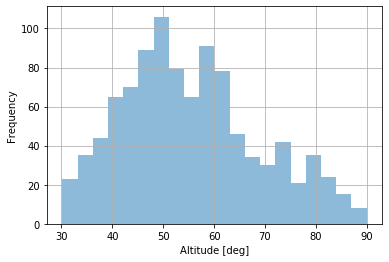
\includegraphics[width=0.495\linewidth]{elevation_distribution.png}
  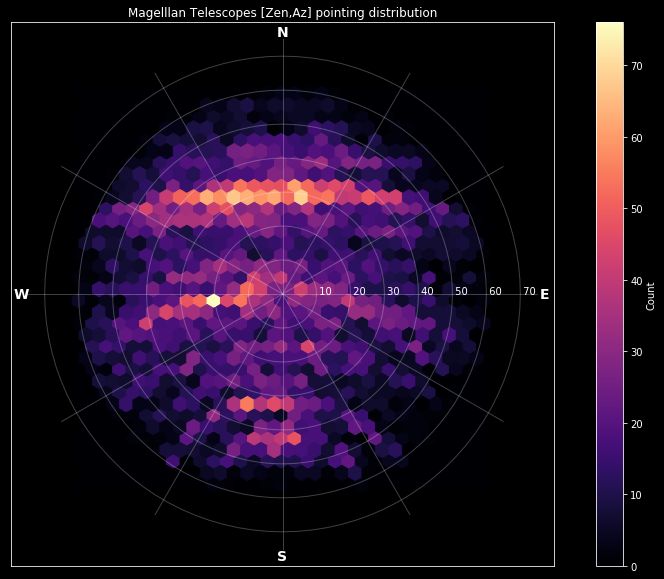
\includegraphics[width=0.8\linewidth]{zenaz_distribution.png}
  \caption{Zenith and azimuth angles distribution from the Magellan telescopes.}
  \label{fig:9}
\end{figure}
We use a collection of 13362 pointing directions of the Baade telescope from
the Magellan observatory to sample the sky accessible to the GMT within a 30 to
90 degrees elevation range.
A 1000 samples are uniformly drawn from the Baade dataset and each sample consists
in an oberving time stamp and an alt--az coordinate.
The observing dates range from 2011 to 2014.
%The 1000 (RA,DEC) sky coordinates are uniformly drawn from a collection of 13362
%pointing directions of the Baade telescope collected from 2011 to 2014.
The RA and DEC distributions of the full and reduced Baade pointing directions are
shown in Fig.~\ref{fig:3}.
\begin{figure}
  \centering
  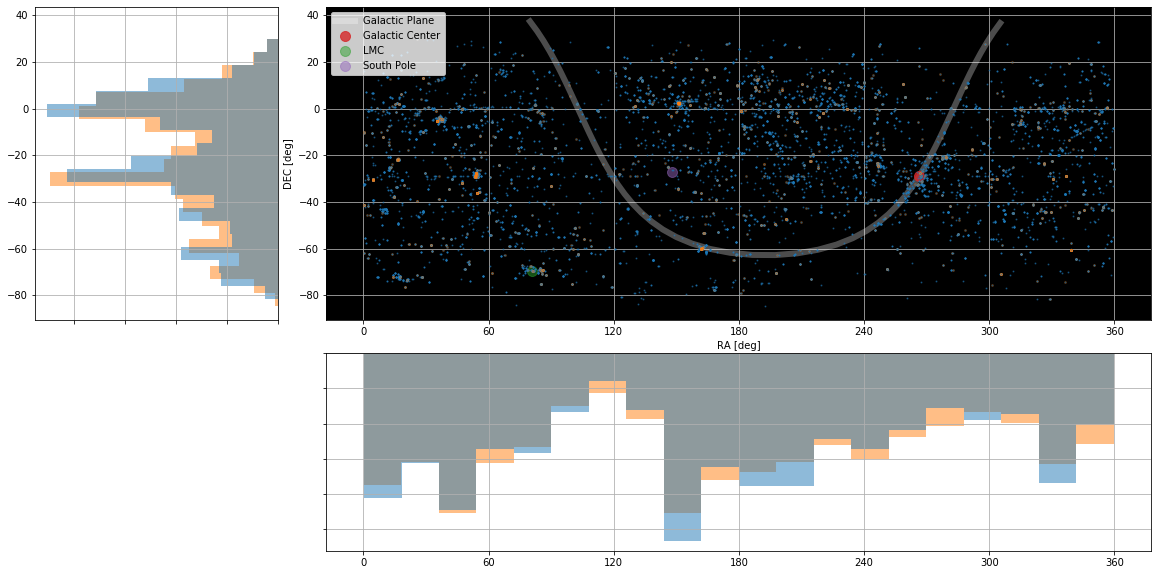
\includegraphics[angle=-90,scale=0.45]{standard_year_Baade_pointing_distribution}
  \caption{RA and DEC distributions of pointing directions for the Baade
    telescope.}
  \label{fig:3}
\end{figure}
The plot shows a higher densities for extra--galactic sources and sources close
to the Galactic Center.

The algorithm that selects the Active Optics guide stars in a given field of
view is detailed in \cite{ATP}. For a given (RA,DEC) coordinates, the algorithm
goes through the following steps:
\begin{enumerate}
\item a 10 arcmin radius circular region is queried from the TESS Input
  Catalogue
  (TIC\footnote{\url{https://tess.mit.edu/data/tess-input-catalogue/}}) centered
  on the specified sky coordinate,
\item the dataset is reduced to stars that have both a V and a J magnitude and
  that are no fainter than V$=18$,
\item the stars are reduced to the ones only accessible to the SH probes (Fig.~\ref{fig:4}),
\item the stars within the radii 6 arcmin and 10 arcmin are
  selected
\item for each star in the down--selected field, one seeks 2 other stars such as
  their angles with respect to the given star is close to 120 degree and -120
  degree, respectively.
If the 2 stars are perfectly symmetric with respect to the given star, then the
sum of both relative angles is zero.
\item for the 10 most symmetric GS triplets, the statistics of
  detector noise propagation (both photon and read--out noise) in the active optics system is evaluated for 10
  samples.
  The final GS triplet is the one with the smallest median wavefront error rms.
\end{enumerate}
\begin{figure}
  \centering
  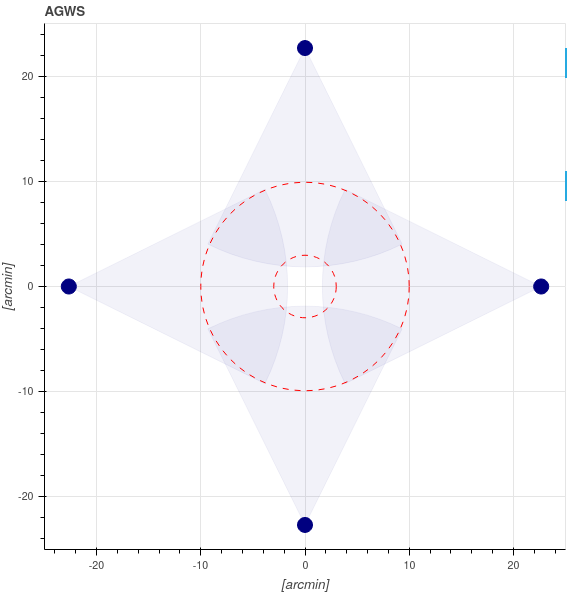
\includegraphics[width=0.45\linewidth]{AGWS_probe_range_layout.png}
  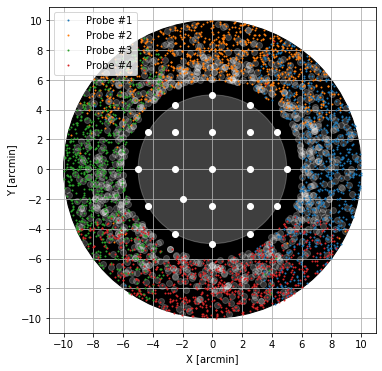
\includegraphics[width=0.5\linewidth]{active_optics_guide_stars.png}
  \caption{AGWS probe patrol ranges (left) and guide stars location for each
    probe (right). The white dots are the locations where the KPPs are estimated.}
  \label{fig:4}
\end{figure}
The algorithm finds suitable asterisms for 99.6\% of the (RA,DEC) sample.
The 996 active optics asterisms are plotted in Fig.~\ref{fig:4} for each of the
AGWS probe. Each asterism is a star triplet as show in Fig.~\ref{fig:5}.
\begin{figure}
  \centering
  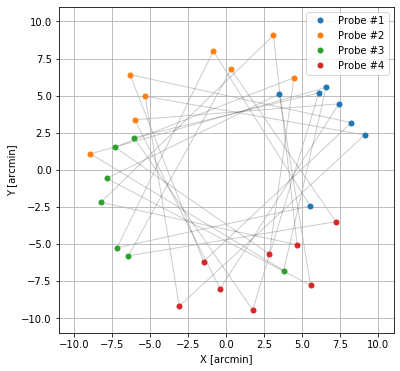
\includegraphics[width=0.495\linewidth]{GS_triplets_few.png}
  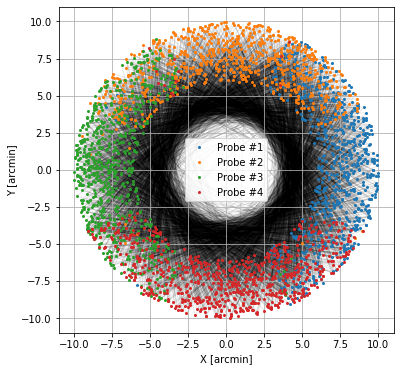
\includegraphics[width=0.495\linewidth]{GS_triplets_all.png}
  \caption{Active optics GS asterisms.}
  \label{fig:5}
\end{figure}
The GS V and $\delta$V  magnitude distributions are shown in Fig.~\ref{fig:6}.
The $\delta$V distribution is the maximum absolute V magnitude difference
between any two stars in an asterism.
\begin{figure}
  \centering
  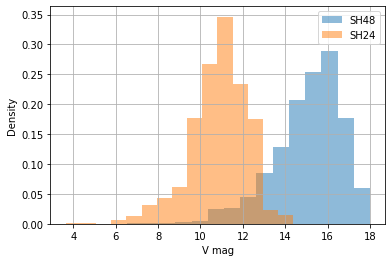
\includegraphics[width=0.495\linewidth]{GS_V_dist.png}
  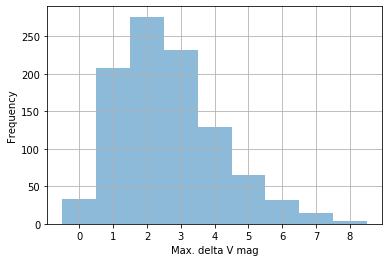
\includegraphics[width=0.495\linewidth]{GS_dV_dist.png}
  \caption{Active optics GS V and $\delta$V magnitude distribution.}
  \label{fig:6}
\end{figure}

\clearpage

\subsection{Atmospheric turbulence}
\label{sec:atm-param}

The turbulent atmosphere is the superposition of several discrete layers with
strong optical turbulence.
Each layer is characterized by the index of refraction structure constant
$C_n^2$ and the wind vector $\vec v$.
We will assume that the 1000 observing cases share the same $C_n^2$ and $\vec v$
profiles but we will associate to each case a unique Fried parameter $r_0$ and
outer scale $\mathcal L_0$.
The $C_n^2$ and $\vec v$ profiles are given in Table~\ref{tab:1} and are based on a median
profile derived from the measurements from Goodwin \cite{Goodwin}.
The parameter $\xi_0$ represents the relative strength of the turbulence in a given layer.
\begin{table}
  \centering
  \begin{tabular}{r|*{7}c}\toprule
    altitude [m] & 25 & 275 & 425 & 1250 & 4000 & 8000 & 13000\\
    $\xi_0$ & 0.1257 & 0.0874 & 0.0666 & 0.3498 & 0.2273 & 0.0681 & 0.0751\\
    wind speed [m/s] & 5.6540 & 5.7964 & 5.8942 & 6.6370 & 13.2925 & 34.8250 & 29.4187\\
    wind direction [rd] & 0.0136 & 0.1441 & 0.2177 & 0.5672 & 1.2584 & 1.6266 & 1.7462\\\bottomrule
  \end{tabular}
  \caption{Turbulence profile}
  \label{tab:1}
\end{table}

For $r_0$, we use the seeing ($\varepsilon_0=0.9759\lambda/r_0$) measurements at the Magellan observatory collected
between 2005 and 2009.
\begin{figure}
  \centering
  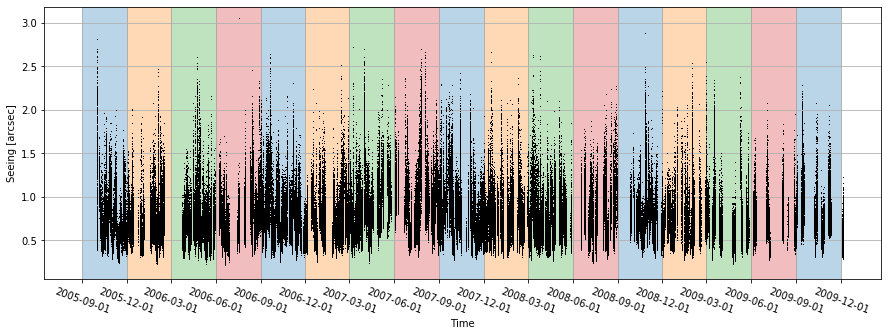
\includegraphics[width=\textwidth]{seeing_seasoned.png}
  \caption{Magellan telescopes seeing dataset.}
  \label{fig:7}
\end{figure}
The seeing dataset is shown in Fig.~\ref{fig:7} with color coded seasons: blue, orange,
green and red corresponding to Spring, Summer, Fall and Winter, respectively.
Some observatories exhibit seasonal seeing variations due to variation in the
turbulence ground layer spurred by change in the direction of the predominant
wind direction.
The Magellan observatory do not show any obvious seasonal pattern,
consequently we will derive $r_0$ from the distribution of the entire dataset.
The seeing distribution is given in Fig.~\ref{fig:8} (left) and it is fitted with a log-normal
distribution.
% We then use this distribution to draw 1000 seeing values, one for each observing case.
The KPP are defined for 15mn long science exposure during which both $r_0$ and $\mathcal L_0$ are expected to vary.
The DIMM measures $r_0$ for continuous period of time ranging from several
minutes to several hours.
During these uninterrupted  measurement periods, $r_0$ is sampled every minute.
From the DIMM records, we have selected all the continuous time series lasting 15mn or more and split them in 15mn long shorter timeseries, as shown in Fig.~\ref{fig:10}.
Then 1000 short time series were randomly affected to each observing case.
The histogram of the mean values of the 1000 seeing 15mn time series is plotted in Fig.~\ref{fig:11} and compared to the distributions of the entire seeing record and of the mean values of the seeing of all the short time series.
We have also computed the variability of the seeing within each 15mn time series as the ratio between the seeing peak--to--valley and the seeing 15mn average. The variability histogram is plotted in Fig.~\ref{fig:11}, the median value is 32\%.

\begin{figure}
  \centering
  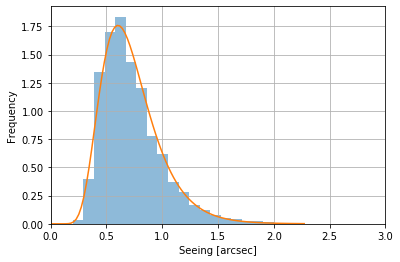
\includegraphics[width=0.495\textwidth]{seeing_distribution.png}
  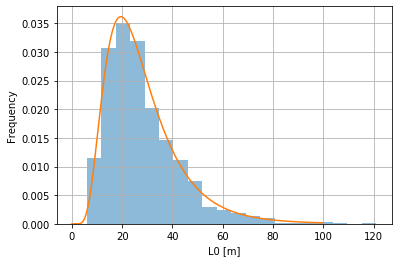
\includegraphics[width=0.495\textwidth]{L0_distribution.png}  
  \caption{Seeing (left) and outer scale (right) distributions.}
  \label{fig:8}
\end{figure}

There is not record of the outer scale $\mathcal L_0$ at the Magellan site.
But $\mathcal L_0$ measurements at other observatories \cite{myself} have
recorded log--normal $\mathcal L_0$ distributions with  median values
consistently at about 25m and with values as low as 5m.
So we have created a log--normal $\mathcal L_0$ distribution with a 25m median
and used the distribution to draw 1000 $\mathcal L_0$ values to complement
the $r_0$ value of each case.
Both the log-normal distribution and the $\mathcal L_0$ histogram are shown in
Fig.~\ref{fig:8} (right).
$\mathcal L_0$ values will remain constant during the whole simulation.


\begin{figure}
  \centering
  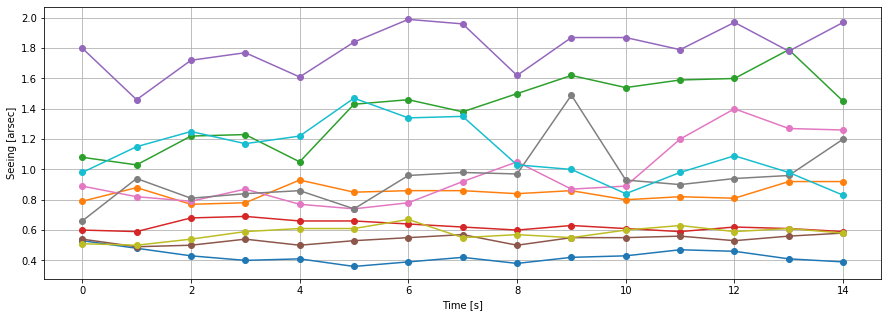
\includegraphics[width=\linewidth]{seeing_15mn_timeseries.png}
  \caption{15mn seeing time series}
  \label{fig:10}
\end{figure}

\begin{figure}
  \centering
  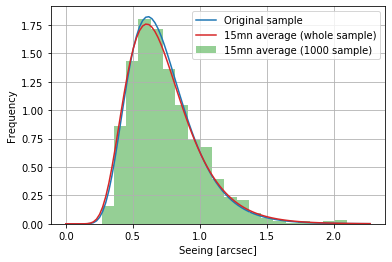
\includegraphics[width=0.495\linewidth]{seeing_15mn_timeseries_stats.png}
  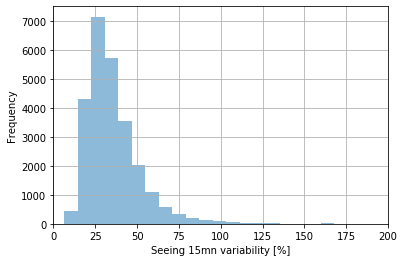
\includegraphics[width=0.495\linewidth]{seeing_variability.png}
  \caption{Left: histogram of the mean seeing values of the 1000 seeing 15mn long time series compared to the seeing distribution of the entire seeing record. Right: 15mn seeing time series variability}
  \label{fig:11}
\end{figure}

\paragraph{Numerical implementation} ~\\
The $r_0$ for the atmosphere is given at zenith and for $\lambda_{r_0}=500$nm.
Hence for each observing case, $r_0$ is scaled according to the pointing zenith
angle $z$: $r_0(z)=r_0(0)(\cos(z))^{3/5}$ and to the wavelength of
the guide star: $r_0(\lambda)=r_0(\lambda_{r_0})(\lambda/\lambda_{r_0})^{6/5}$.
\marginpar{\small wind speed and layer altitude need to scaled with $z$ as well}

All the phase screens are pre--computed using a default $r_0$ value ($r_0=15$cm)
and for each observing case and each guide star the phase screens are scaled to
the proper $r_0(z,\lambda)$.
In the telescope pupil, the phase screens are computed over a $26\times26$m
square area with a 2cm spatial sampling in both x and y directions.

Phase screens cannot be scaled with $\mathcal L_0$.
So 18 phase screens were pre--computed with different $\mathcal L_0$ regularly
spanning the range [5--90]m.
For each observing case, the phase screens with $\mathcal L_0$ the closest to the
$\mathcal L_0$ associated to the case is selected.


\subsection{Dome seeing and wind shake}
\label{sec:CFD}

\begin{table}
  \centering
  \begin{tabular}{ll}\\
    Zenith [degree] & : 0,30,60 \\
    Wind Speed [m/s] & : 2,7,12,17 \\
    Azimuth [degree] & : 0,45,90,135,180
  \end{tabular}
  \caption{CFD cases parameters}
  \label{tab:1}
\end{table}
\begin{table}
  \centering
  \begin{tabular}{cc@{  (}cc@{)}}
    Vents & Wind screen & Wind speed [m/s] & zenith [degree] \\\hline
    open & stowed & 2,7 & 0,30,60 \\
    closed & deployed & 12,17 & 0,30\\
    closed & stowed & 12,17 & 60 
  \end{tabular}
  \caption{Enclosure configurations}
  \label{tab:2}
\end{table}

Dome seeing and wind loads (forces and moments) on the telescope structure were computed using computational fluid dynamics (CFD) simulations for 60 different telescope enclosure and wind speed configurations.
The telescope is setup with 3 elevation 90, 60 and 30 degrees and for each elevation, there are 5 different enclosure orientation with respect to the direction of the predominent wind: 0, 45, 90, 135 and 180 degrees.
For each combination of elevation and azimuth parameters, the simulations are repeated 4 times, each time with a different wind speed: 2, 7, 12 and 17 m/s.
For 2 and 7 m/s cases, the enclosure vents are open and the wind screen is stowed, whereas for the 12 and 17 m/s cases, the vents are closed and the wind screen is deployed.

\begin{figure}
  \centering
  %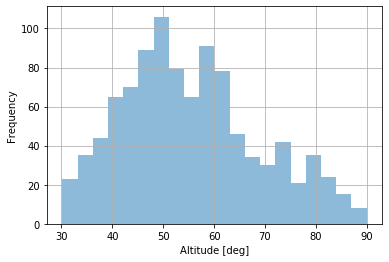
\includegraphics[width=0.495\linewidth]{elevation_distribution.png}
  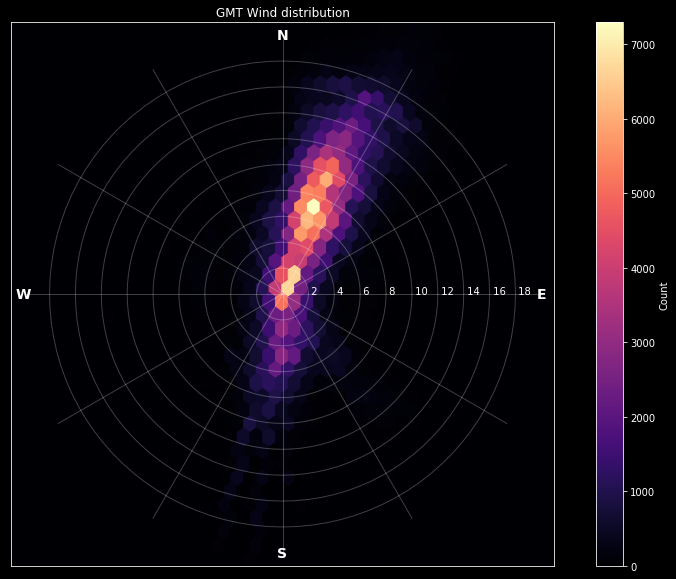
\includegraphics[width=0.8\linewidth]{wind_distribution.png}
  \caption{Wind vector distribution measured at the GMT site.}
  \label{fig:9}
\end{figure}

A wind speed of either 2, 7, 12 or 17m/s is randomly affected to each observing case in a round--robin fashion such as there is an equal share of wind speed among the 1000 observing cases.
For each observing case, we select the dome seeing and the wind loads with the elevation and azimuth the closest to the elevation and azimuth of the observing case.
None of the CFD time series last 15mn, so we play the time series forward then backward and the pattern is repeated until the 15mn mark is reached.

% \subsection{PSSn stochastic definition}
% \label{sec:stochatic-pssn}

\subsection{Pupil rotation}
\label{sec:pupil-rotation}

As the telescope tracks a target in the sky, from the point of view of an
observer on the telescope, the whole sky rotates around the target.
The angular rotation speed $\dot{p}$ is a function of the latitude of the observatory $l$,
the alt-az $(a,A)$ coordinates of the telescope and the sideral rate $\omega_0=15$arcsec/s:
\begin{equation}
  \label{eq:9}
  \dot{p} = w_0{\cos(l)\cos(A)\over\cos(a)} arcsec/s.
\end{equation}
The AGWS and the instruments at the direct and folded focal stations of the telescope are
located on the Gregorian Instrument Rotator (GIR) that rotates at the same
angular rate $\dot p$ than the sky.
Consequently, an observer now located on the GIR, will see the sky in a
standstill but with the telescope rotating around him.
In the GIR relative frame of reference, the optical conjugate of the telescope
entrance pupil (given by M1) is then rotating
%\marginpar{\small what about nutation? (AGWS 15\% of subaperture)}
at the same rate than the GIR.

As the telescope tracks, altitude $a$ and azimuth $A$ varies at the following speed:
\begin{eqnarray}
  \label{eq:10}
  \dot{a} &=& -w_0\sin(A)\cos(l),\\
  \dot{A} &=& w_0(\sin(l)+\tan(a)\cos(A)\cos(l)).
\end{eqnarray}
The discrete time equation of the rotator angle $p$, altitude $a$ and azimuth $A$ are
\begin{eqnarray}
  \label{eq:11}
  p_{n+1} &=& p_n + \dot{p_n}\tau,\\
  a_{n+1} &=& a_n + \dot{a_n}\tau,\\
  A_{n+1} &=& A_n + \dot{A_n}\tau,
\end{eqnarray}
where $\tau$ is the sampling period.
$a_0$ and $A_0$ are given by the coordinates of the target when tracking starts.
$p_0$ is given by the parallactic angle:
\begin{eqnarray}
  \label{eq:12}
  \tan(p) = {\sin(H)\over \tan(l)\cos(\delta) - \sin(\delta)\cos(H)},
\end{eqnarray}
with $\delta$, the target declination and $H$, the hour angle given by
$H=t_0-\alpha$ where $t_0$ is the sideral time and $\alpha$ the target right
ascension.

The histograms of the amount of parallactic ($p$), elevation ($a$) and azimuth ($A$) angle
variation during 15mn of mount tracking are given in Fig.~\ref{fig:12},
Fig.~\ref{fig:13} and Fig.~\ref{fig:14}, respectively.

\begin{figure}
  \centering
  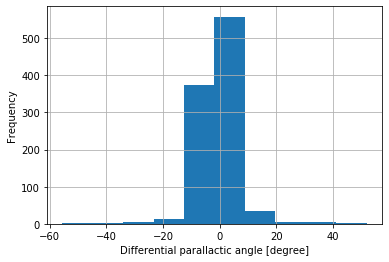
\includegraphics[width=0.55\textwidth]{diff_p_angle.png}
  \caption{Amount of parallactic angle variation for a 15mn mount tracking
    duration.}
  \label{fig:12}
\end{figure}

\begin{figure}
  \centering
  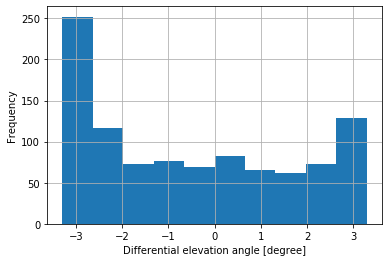
\includegraphics[width=0.55\textwidth]{diff_el_angle.png}
  \caption{Amount of elevation angle variation for a 15mn mount tracking
    duration.}
  \label{fig:13}
\end{figure}

\begin{figure}
  \centering
  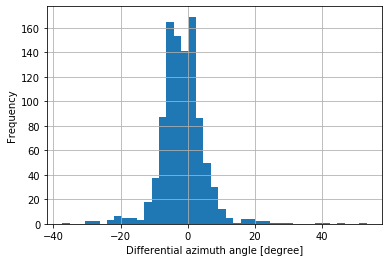
\includegraphics[width=0.55\textwidth]{diff_az_angle.png}
  \caption{Amount of azimuth angle variation for a 15mn mount tracking
    duration.}
  \label{fig:14}
\end{figure}

\subsection{Night time temperature}
\label{sec:night-temp}

\begin{figure}
  \centering
  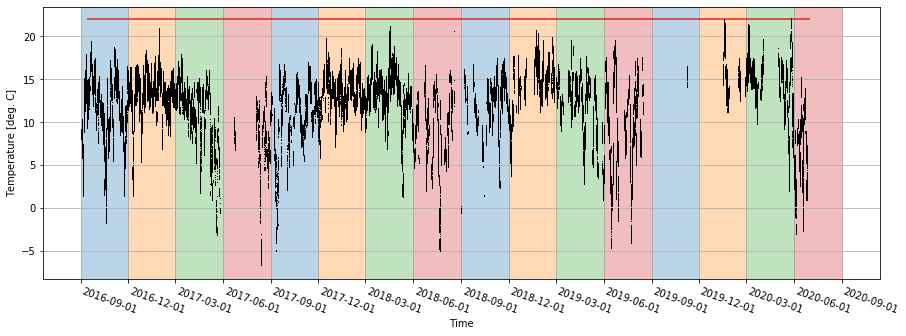
\includegraphics[width=\linewidth]{temperature_seasoned.png}
  \caption{Night time temperature at GMT site.}
  \label{fig:1}
\end{figure}

\begin{figure}
  \centering
  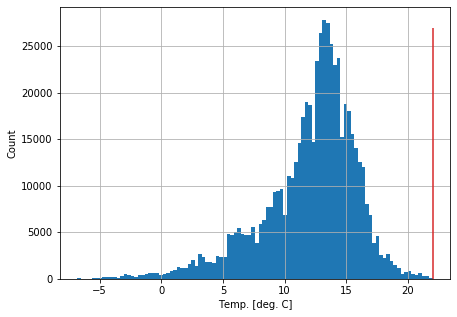
\includegraphics[width=0.495\linewidth]{temperature_distribution.png}
  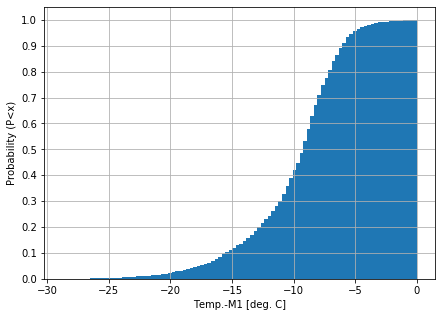
\includegraphics[width=0.495\linewidth]{temperature_M1_cumdist.png}
  \caption{Night time temperature distribution at GMT site.}
  \label{fig:2}
\end{figure}

\printbibliography

\end{document}
